\label{conclusions}
This section presents a summary of the results from previous chapters, compares
our results with LaMarca's, lists important results and discoveries, and
suggests contributions made to computer science by this research.

\section{Results summary}

\subsection{Elementary Sorts}

We found that insertion sort has the best performance of any of the elementary
sorts, with fewer instructions, cache misses and exactly one branch
misprediction per key. Selection sort also has very few branch mispredictions,
and our results match Knuth's calculations. We find that reducing the number of
runs in bubblesort and shakersort at the cost of additional instructions is
counter productive, and that their branch prediction performance is incredibly
poor.

\subsection{Heapsort}

The cache optimized heaps perform better than the non-optimized versions. At the
cost of a slightly increased instruction count, the number of branch misses can
be greatly reduced, and the overall performance of our 8-heap is significantly
better than the unoptimized version. This is despite our finding of that
increasing the fanout increases branch mispredictions.

Additionally, we created an improvement to heapsort which removed the need for a
sentinel, without introducing any more instructions.

\subsection{Mergesort}

We found that algorithm S has a lower instruction count than algorithm N, but
that this does not necessarily translate to better performance. Our results show
also that the level 1 cache needs to be taken into account, that the extra
instruction in multi-mergesort make it slower than double-aligned tiled
mergesort, and that multi-mergesort has regular branch predictive access
patterns during the k-way merge, which can be taken advantage of by a 2-level
adaptive predictor.


\subsection{Quicksort}

Our results show base quicksort being the fastest of the quicksorts. We note our
lowest instruction count occurs with the median-of-7 partitioning. We also see
that using a binary search slows multi-quicksort down compared to a sequential
search, but that its extra instructions make it slower than memory-tuned
quicksort.  Despite being slower in our tests, our simulations show tuned
quicksort to have fewer cache misses, instructions and branch mispredictions
than base quicksort.

\subsection{Radixsort}

We were able to reduce the number of cache misses considerably using a technique
adapted from LaMarca's tiled mergesort, and managed to make memory-tuned radixsort the
fastest sort in our tests. This is due to its low instruction count, few cache
misses and lack of branch mispredictions. Although we attempted to align it
using another technique from mergesort, we found this decreased its performance.

\subsection{Shellsort}

Based on our tests, shellsort performs very similarly to an $O(NlogN)$ sort,
outperforming heapsort. We note that our improved version is considerably
faster, mostly due to its reduced instruction count.

We were also able to measure it's branch mispredictions, and determine a formula
to calculate them.

\section{Branch Results}
%TODO this section has to be reread by David

No results for the branch prediction performance of sorting algorithm yet
exists. We discovered some interesting new results.

Insertion sort has exactly one miss per key. Using this result we were able to
make several other sorts faster by replacing their simple inline sorts with
insertion sorts.

Selection sort also has a very low number of branch mispredictions, the results
of which match up well to Knuth's calculation. We found as well that bubblesort
and shakersort have incredibly bad branch prediction performance. Both are
$O(N^2)$ sorts, and the number of branches and branch misses have the same
complexity.
%TODO i dont like how this reads

TODO bubblesort

In heapsort, we found a pattern of branch mispredictions when using a fanout in
our 8-heap, and that this pattern matched closely that of selection sort,
discussed above. Despite this property, the number of mispredictions using an
8-heap was greater than when using a 4-heap.

Using a k-way merge, multi-mergesort had a great number of extra branch
predictions. While many of these were mispredicted using the bimodal predictor,
the 2 level adaptive predictor was able to predict a higher
proportion correctly.


TODO quick

TODO radix

TODO shell


%TODO results from software predictors

\section{Comparison with LaMarca's Results}

Over the course of this research. The vast majority of our results have
correlated exactly with LaMarca's. Many of our graphs are exactly the same
shape to LaMarca's, can be calculated exactly or almost exactly using his
methods, or can be seen to be equivalent when scaled by an appropriate ratio
(due to different test parameters).

LaMarca's heapsort graphs were equivalent to ours in the areas of level 1
misses, instruction count and cycle count. Like LaMarca, we found that a four
heap lowered our instruction count. Our level 2 misses also concurred with
LaMarca, with only one difference: memory-tuned heapsort, being an out-of-place sort,
fills the cache fully with a smaller number of keys than base heapsort, which is
in place. LaMarca's results do not show this. Nor do they show a difference in
cache misses between these two sorts when the array does fit in the cache.
LaMarca's base heapsort have the characteristics of an out-of-place heapsort.
However, our results show that his implicit heap improvements have led to a
significantly faster heapsort.

LaMarca's initial improvements to base mergesort were due to reduce the
instruction count. We noted a reduction with each of the steps he prescribed. We
note too that each of his improvement reduce level 2 cache misses, and the shape
of our level 2 cache miss graphs exactly match his. We also note similar
characteristics: LaMarca mentions a wobble in the instruction count graphs, due to
having to copy the final merge back; we note this same wobble.

However, we disagree with his results in several key places. Firstly, we note
that an in-lined sorting method does not perform as fast as insertion sort. We
find it difficult to perform his improvements on either algorithm N or algorithm
S, and write our own mergesort instead. We expected that mergesort would have
half the instruction count of heapsortl we found instead they were very similar.

LaMarca did not include details of his tagging system in multi-mergesort. As a
result, we used a search, which greatly increased the instruction count. As a
result, multi-mergesort did not perform as well as the mergesorts which had only
been tiled. 

We note also that aligning the level 2 cache alone leads to worse
performance than not making any improvements at all, due to the thrashing of the
level 1 cache. When we aligned the arrays for the level 1 cache, the results
were much closer to LaMarca's results, and showed what an improvement his
techniques brought to those algorithms.


Our quicksort results, again, we very similar to LaMarca's. We showed an
increase is instruction count of 25\% due to multi-quicksort - very close to
LaMarca's 20\%.  The shape of our instruction count graphs were the same, and
switching to a binary search in multi-quicksort reduces the instruction count.
Like him, we found that the base quicksort had very few cache misses, and that
not using Sedgewick's insertion sort improvement reduces cache misses. We found
that multi-quicksort's k-way sort changes the slope of the graph, but our
result were not conclusive as to whether this would eventually make
multi-quicksort faster than the other versions. Our results do show it being
slower for all our test cases, due to the increase in instruction count.

LaMarca predicts two cache misses per key, which translated to one miss per key
with our 32 bit integers. We found this calculation to be true, as is his
calculation of a decrease of one cache miss in four: we note a reduction of one
cache miss in eight.

Where LaMarca found that using Sedgewick's insertion sort optimisation decreased
instruction count, we found the opposite. We also found that despite
improvements due to cache performance and instruction count, our base quicksort
performed faster than our memory-tuned version. Finally, we found that although
changing multi-mergesort's sequential search to a binary search decreased the
instruction count, it greatly increased the number of branch mispredictions
incurred, and slowed the sort down accordingly.

LaMarca determines that radixsort could not be improved in the same was as the
comparison-based sorts, and that due to poor cache performance, it ran more
slowly than quicksort. We showed, however, that one of the improvements applied
to mergesort could be applied to it, and that its resulting cache performance is
sufficiently good that its low instruction count and lack of branch
mispredictions make it the fastest sort in our survey.


\section{Important results and contributions}

%TODO lamarca does an overall comparison. we should do the same

\section{Instruction count results}

\section{Cache Results}

% TODO more details in this
The test results in this project mostly agreed with LaMarca's results.  The
heapsort graphs had nearly exactly the same shape as LaMarca's, and the ratios
between the base and cache-conscious versions were nearly identical. The
multi-mergesort results were slightly different: instruction count was
identical, but while the cache results of the base and tiled mergesorts were
identical, multi-mergesort results were not the same. However, the basis for
those results - a sharp increase in cache misses followed by a flat-lined graph
- were in both cases.

The quicksort results were also very similar, though the multi-quicksort results
had a very different shape to LaMarca's. However, the instruction count
results for each quicksort agreed with LaMarca's results, as did cache miss
results of the base and cache-conscious versions.

The two sets of radixsort results were slightly similar. The rise and plateau of
the curve to the right of the graphs was the same in both cases, though the left
hand side of the graphs did not agree.

Another interesting observation can be made: the results of the simulations on
the Pentium 4 were not always influenced by the cache misses. Though heapsort
and radixsort began to perform poorly once the data set no longer fit in the
cache, neither quicksort nor mergesort were affected. The reason why radixsort
was affected is obvious - there is no temporal reuse; in heapsort, the full
cache line is not being used, and spatial locality suffers as a result. It is
interesting that the other two sorts were unaffected, even though their cache
miss graphs indicate a significant increase in misses.

Finally, it was shown that in some cases a direct-mapped cache performed better
than a fully-associative one. The reasons for this were not clear.

\section{Branch Prediction Results}

Insertion sort has only one branch misprediction per key. This shows that it is
possible to predict comparative branches correctly, though the instruction cost
of such an algorithm may be high. This is also shown in multi-quicksort: though
the instruction count and memory reference count are both doubled, it is still
faster to use a sequential search than a binary search across small lists.

Selection sort has a similar number of instructions and cache misses as
bubblesort and a larger instruction and cache miss count than shakersort, yet it
still considerably outperforms both of these. This shows the high cost of branch
mispredictions on an algorithm.

Radixsort has almost no branch mispredictions at all. The only mispredictions
are due to its flow control, but it escapes comparative mispredictions, and this
factor allows it to perform as fast as, and in some cases faster than quicksort,
despite its high number of cache misses.

The heapsort results show the disadvantage of using unsorted lists. Even though
there are less branches in the 4-heap version, the number of branch
mispredictions are higher than in a standard 2-heap.

It is also shown that bimodal branch predictors generally out-perform two-level
adaptive predictors when resolving comparative misses. This is shown by the
results of insertion sort, bubblesort, shakersort, heapsort and quicksort. In
the cases where the two-level adaptive predictor does perform as well, the table
required is much larger than that required by the bimodal predictors to get the
same results.

\section{Best Sort}
The results also helped answer the question of which is the best sort. However,
it is important to remember that sorts have different purposes and properties,
so this shall be considered. A comparative chart of the fastest sorts is shown
in Figure \ref{All cycles}. This shows the cycles per key of each of the major
sorts and their derivatives, measured using Pentium 4 performance counters.
None of the elementary sorts or heapsorts are on the chart, as their results
are significantly worse than the other results, which makes it difficult to
accurately see them.

\afterpage{
\thispagestyle{empty}
\clearpage
\enlargethispage{14em}
\vspace*{-10em}
\setcounter{figure}{9} % note the cheating to make this work
\begin{figure}[H]
\begin{changemargin}
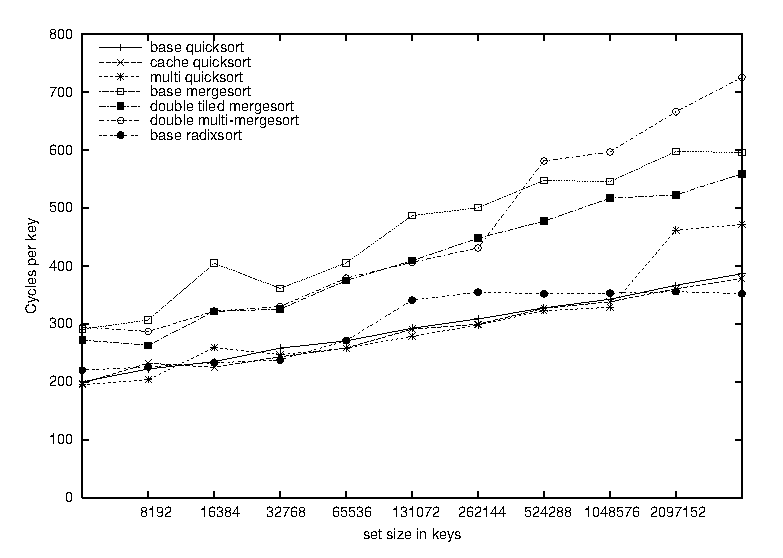
\includegraphics[angle=90,scale=1.8]{plots/all_cycles}
\vspace*{8em}
\end{changemargin}
\caption[Cycles per key of several major sorts and their variations]{\label{All
cycles}Cycles per key of several major sorts and their variations - this was
measured on a Pentium 4 using hardware performance counters.}
\end{figure}
\newpage
}

The best stable sort is radixsort. The best comparison-based stable sort is
double-aligned tiled mergesort. The best in-place sort is quicksort. The best in-place
stable sort is, sadly, insertion sort. The best elementary sort is also
insertion sort; as such it should be only used for very small data sets.  The
best sort for very large data sets is radixsort. The fastest overall sort was
memory-tuned radixsort, though quicksort is very close.
% TODO redo above paragraph

\section{Contributions}

This section lists the contributions of this project. Each of these is novel  
and was discovered or developed during the course of this project.

The primary contribution of this project is that it repeats the work of LaMarca
on cache-conscious sorting, and validates many of his claims, while questioning
others. The next most important contribution is having performed a branch
prediction analysis of major sorts - which to my knowledge has not been done
before - and developing a framework by which these results can be repeated and
expanded upon.

%TODO claims that it backed
% TODO claims that it refuted or found problems with
% - cache in heapsort
% - algorithm N, can those improvements really be made

Several discoveries were made and analysed: insertion sort has one misprediction
per key; selection sort has $log_2(N/2)$ branch mispredictions per key - an
explanation of this was also provided; tiling mergesort can be done in two
steps, reducing the cache miss count; it is possible to avoid using a
sentinel and still remove the bounds check from a standard 2-heap, simply by
reordering the steps involved; sequential searches are far cheaper than binary
searches across small lists, due to a low branch misprediction rate.

%TODO add novel contributions
% - avoid copying back in mergesort
% - remove bounds check without sentinel in base heapsort
% - double-tiling


%TODO look over these
In addition, several ideas were conceived although not implemented, which relate
to sorting algorithms: it should be possible to reduce the conflict misses of
tiled mergesort without padding, by slightly reducing the size of the array
segments sorted in the first sorting phase; it may be possible to reduce the
cost of an insertion sort or selection sort by considering more than one key at
a time; it may be possible to reduce the number of partitions - and hence the
increase in instruction count - of multi-quicksort by choosing from a larger
selection of pivots. Finally, it should be possible to reduce by half the number
of cache misses in radixsort, by counting earlier and by copying back and forth
between two arrays.
